
% Include LaTeX packages
\documentclass[conference]{styles/acmsiggraph}
\usepackage{comment} % enables the use of multi-line comments (\ifx \fi)
\usepackage{fullpage}
\usepackage{enumitem}
\usepackage{amsmath,amsthm,amssymb}
\usepackage{listings}
\usepackage{minted}
\usepackage{graphicx}
\usepackage{etoolbox}
\usepackage{verbatim}
\usepackage[dvipsnames]{xcolor}
\usepackage{fancyvrb}
\usepackage{hyperref}
\usepackage{menukeys}
\usepackage{titlesec}
\usepackage{csquotes}
\usepackage{placeins}
\usepackage{algorithm} 
\usepackage{algpseudocode}
\usepackage{booktabs}
\usepackage{unicode-math}
\newcommand{\?}{\stackrel{?}{=}}
\renewcommand\qedsymbol{$\blacksquare$}

% Set additional LaTeX options
\setlength{\parskip}{.8mm}
\setcounter{MaxMatrixCols}{20}
\hypersetup{
	colorlinks=true,
	urlcolor=[rgb]{0.97,0,0.30},
	anchorcolor={0.97,0,0.30},
	linkcolor=black,
	filecolor=[rgb]{0.97,0,0.30},
}

% Define title, author, and affiliation information
\title{\huge Programming Assignment 2 \\ \LARGE {CS124: Data Structures and Algorithms \\ Prof. Mitzenmacher}}
\author{\Large Dhilan Ramaprasad \\
dhilanramaprasad@college.harvard.edu \\
Collaborator: Benny Paris}
\pdfauthor{Dhilan}

% Redefine \VerbatimInput
\RecustomVerbatimCommand{\VerbatimInput}{VerbatimInput}%
{fontsize=\footnotesize,
 %
 frame=lines, % top and bottom rule only
 framesep=2em, % separation between frame and text
 rulecolor=\color{Gray},
 %
 label=\fbox{\color{Black}\textbf{OUTPUT}},
 labelposition=topline,
 %
 commandchars=\|\(\), % escape character and argument delimiters for commands within the verbatim
 commentchar=* % comment character
}

% Set addditional formatting options
\titlespacing*{\section}{0pt}{5.5ex plus 1ex minus .2ex}{2ex}
\titlespacing*{\subsection}{0pt}{3ex}{2ex}
\setcounter{secnumdepth}{4}
\renewcommand\theparagraph{\thesubsubsection.\arabic{paragraph}}
\newcommand\subsubsubsection{\paragraph}

% Define a convenient norm symbol
\newcommand{\norm}[1]{\left\lVert#1\right\rVert}
\renewcommand{\vec}[1]{\mathbf{#1}}

% Define a macro for hiding answers
\newbool{hideanswers} \setbool{hideanswers}{false}
\newenvironment{answer}{}{}
\ifbool{hideanswers}{\AtBeginEnvironment{answer}{\comment} %
\AtEndEnvironment{answer}{\endcomment}}{}

% Define text formatting for points and normals
\newcommand{\points}[1]{\hfill \normalfont{(\textit{#1pts})}}
\newcommand{\pointsin}[1]{\normalfont{(\textit{#1pts})}}







%%%%%%%%%%%%%%%%%%%%%%%%%%%%%%%%%%%%%%%
%%%%%%%%%%%%%%%%%%%%%%%%%%%%%%%%%%%%%%%
%%%%%%%%%%%%%%%%%%%%%%%%%%%%%%%%%%%%%%%
%%%%%%%%%%%%%%%%%%%%%%%%%%%%%%%%%%%%%%%
%%%%%%%%%%%%%%%%%%%%%%%%%%%%%%%%%%%%%%%

         %  START HERE  %

%%%%%%%%%%%%%%%%%%%%%%%%%%%%%%%%%%%%%%%
%%%%%%%%%%%%%%%%%%%%%%%%%%%%%%%%%%%%%%%
%%%%%%%%%%%%%%%%%%%%%%%%%%%%%%%%%%%%%%%
%%%%%%%%%%%%%%%%%%%%%%%%%%%%%%%%%%%%%%%
%%%%%%%%%%%%%%%%%%%%%%%%%%%%%%%%%%%%%%%

\begin{document}
\maketitle

\section{Analytical Cross-over Point:} \label{section:Math}
\textbf{Note:} Collaborated with Benny Paris (prior PA partner and PSET collaborator) and Marwa here. \\

We can start with a recurrence relation for our hybrid form of Strassen
\begin{equation}
  T(n)=\begin{cases}
    7T(\frac{n}{2}) + O(n^2) & n > n_0\\
    O(n_0^3) & n\leq n_0
  \end{cases}
\end{equation}

Given 18 additions, we can more clearly write:
\begin{equation}
  T(n)=\begin{cases}
    7T(\frac{n}{2}) + 18(\frac{n}{2})^2 & n > n_0\\
    O(n_0^3) & n\leq n_0
  \end{cases}
\end{equation}

In our naive matrix multiplication we employ $n_0^3$ multiplications and $(n_0-1)n_0^2$ additions (CMU 750).\\

Remaining naive runtime (at cross-over), then: $2n_0^3 - n_0^2$. \\

\begin{equation}
  T(n)=\begin{cases}
    7T(\frac{n}{2}) + 18(\frac{n}{2})^2 & n > n_0\\
    2n_0^3 - n_0^2 & n\leq n_0
  \end{cases}
\end{equation}

At the cross-over point, we call the upper recurrence once but instead of dividing by 2, and recursively propagating, we switch to the cost of the naive multiplication on a divided matrix and should optimize our crossover such that its dimension, $n$ equals that which we insert into the upper recurrence:

$$2n_0^3 - n_0^2 = 7\left ( 2\left (\frac{n_0}{2}\right )^3 - \left (\frac{n_0}{2}\right )^2\right ) + 18\left (\frac{n_0}{2} \right )^2 $$

$\implies \mathbf{n_0^* = 15}$
\section{Experimental Cross-over Point:} \label{section:PART2}
\subsection{Finding $n_0'$:} \label{section:BIGDATA}

\begin{figure}[h!]
    \centering
    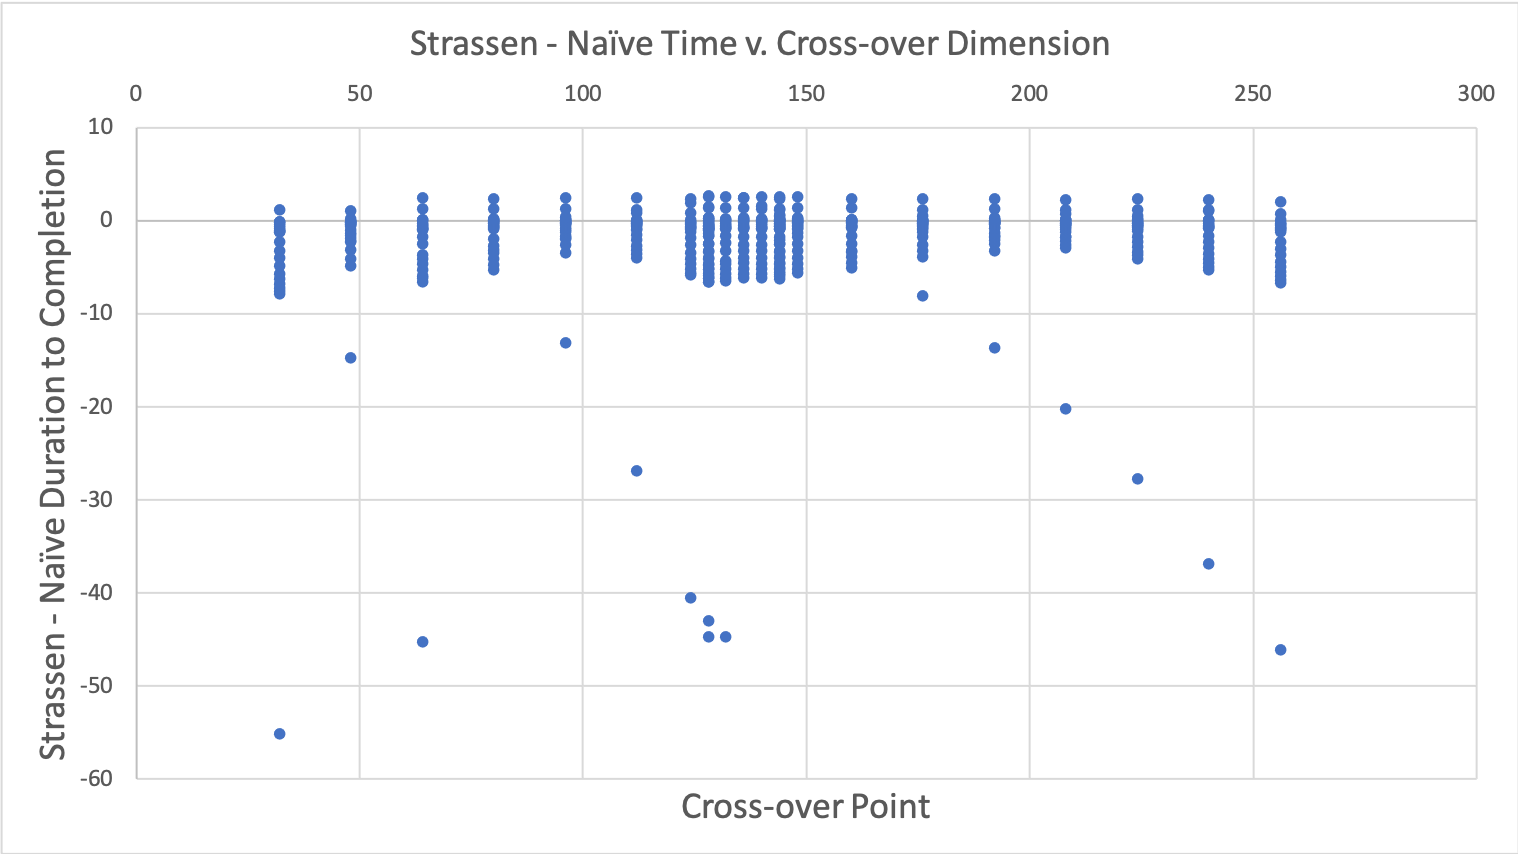
\includegraphics[width=0.7\textwidth]{Figures/broadSearch.png}
    \caption{Varied trials over many selections of $n0$ and input dimension, $n$}
    \label{fig:Cursory Glance}
\end{figure}
\FloatBarrier % this makes sure the image goes right here.

At a cursory glance, two hot-spots were clear: the mid-30s as well as the low-to-mid 100s.  I performed a more detailed repetition of the trials with both varied dimensions at finer grain and matrices filled with different values (uniform distribution of [-1,1], [0,1], and [-20,20]).\\

\begin{figure}[h!]
    \centering
    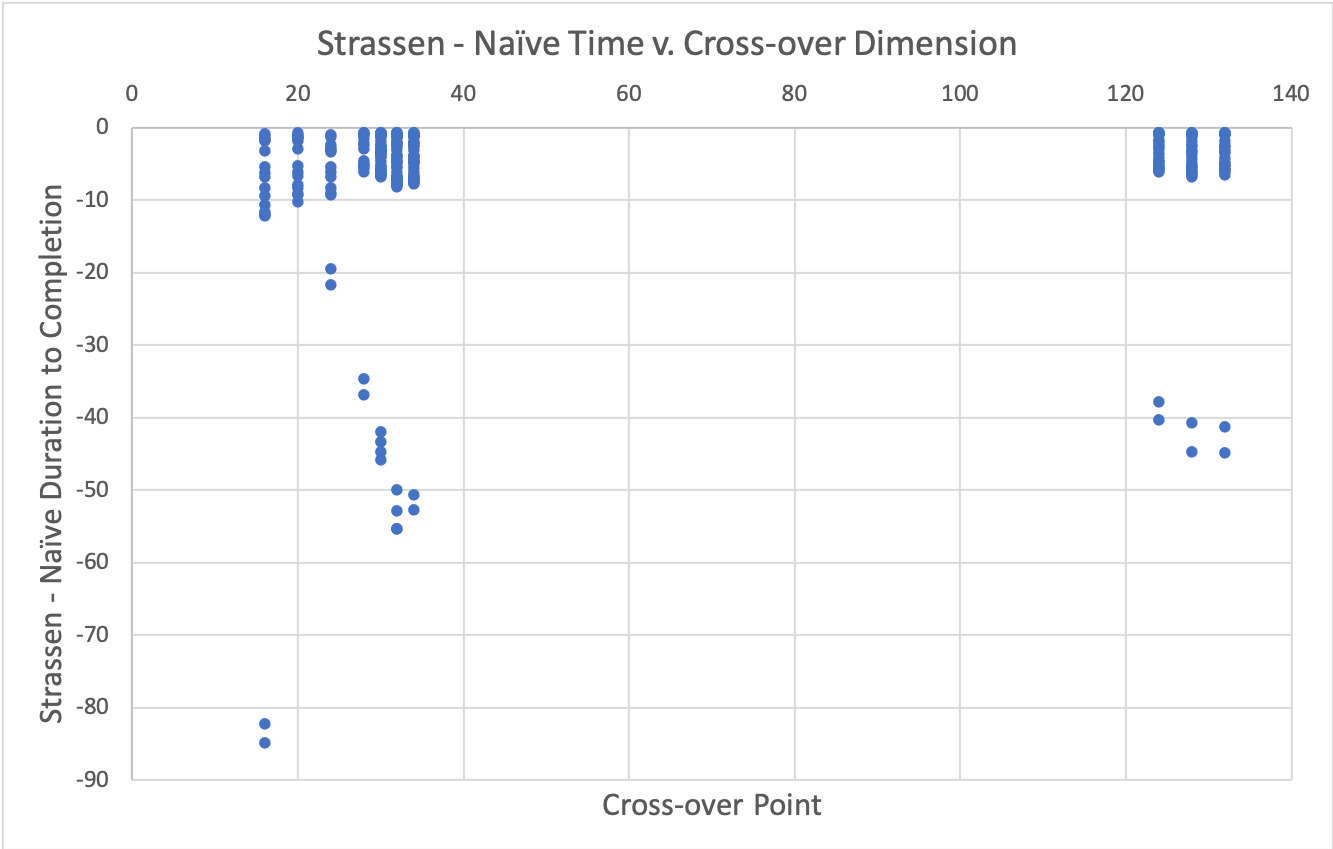
\includegraphics[width=0.7\textwidth]{Figures/Optimal.png}
    \caption{Varied trials over narrowed selection of $n0$ but wider selection of input dimension, $n$}
    \label{fig:Narrowed Search Glance}
\end{figure}
\FloatBarrier % this makes sure the image goes right here.

The close performance of three disparate cross-over points [16, 32, 128] leads me to believe that there are some machine-dependent factors at play here.  Micro-architecturally speaking, perhaps pre-fetch streams, caching mechanisms, and more allow a spike to high performance at the larger dimensions and with the lower dimension cross-over point.  In all, 16, 32 and 128 tended to top the charts in performance (metric: \textbf{most frequent occurrences in top 20 Strassen--Naive difference}).  I did not include raw data here, but would be happy to provide it via email. \\

\textbf{Selection:} $\mathbf{n_0' = 32}$\\
This may change depending on performance on grading server performance as it is machine specific.\\
It is also worth noting that \textbf{\textit{124}} showed up frequently.  Coincidence?  I think not.

\subsection{Reasoning:}
So there are many factors at play here.  (1) Padding is not a \enquote{free} operation.  In fact, it costed quite a bit in some of my initial implementations wherein I was copying data (unnecessarily).  (2) Division into submatrices is not a \enquote{free} operation, and replication / initialization of additional matrices creates a large overhead.  (3) Recombination of matrices is also not a free operation.  After breaking into 4 segments of n/2, the process to \enquote{glue} the product matrix together (recursively) requires a non-trivial amount of time.\\

This said, I was able to achieve close to theoretical without a highly optimized implementation.  This is likely due to a powerful machine optimized at a microarchitectural level.\\

My trials were thorough, so I would like to run more analyses, but I did try odd dimensions, evens, primes, powers of 2, and more, and varied the random input to my multiplicand and multiplier to be on different uniform distributions.\\

In all, there are many more intricacies to the process of determining the cross-over.  Odd numbers (and ensuing padding time), anomalies when it comes to closeness to powers of two rather than multiples of $n_0$ and 2, and more create difficulties to capture a perfect heuristic for when Strassen's is \textit{always} better.

\subsection{Testing methodology:}
For characterization of the best experimental $n_0'$, I ran batches of trials via a bash script which probed cross-over points of size 32-256 shown in preliminary findings in Section \ref{section:BIGDATA} above.  Within those trials, I tested various dimensions of input matrices from 260-1060 at first and then when narrowing in on the ideal cross-over, I tested more values with a focus on odds, primes, and multiples of 2 but not necessarily powers of 2 or multiples of the candidate $n_0'$ and 2.

\section{Triangle in Random Graph:} \label{section:Triangles}
\subsection{Results:}

% Table generated by Excel2LaTeX from sheet 'Part 3'
\begin{table}[htbp]
    \centering
    \begin{tabular}{rccccc}
          &       &       & Probability &       &  \\
        \cmidrule{2-6}          & 0.01  & 0.02  & 0.03  & 0.04  & 0.05 \\
        \cmidrule{2-6}    Expected \# Triangles & 178.43302 & 1427.464 & 4817.692 & 11419.71 & 22304.13 \\
    Experimental \# Triangles & 183   & 1407  & 4818  & 11494 & 22404 \\
        \cmidrule{2-6}    \end{tabular}%
  \label{tab:triangles}%
\caption{Results of 7 Trials Run with Strassen's MM Algorithm}
\end{table}%

\subsection{Methodology:}
I created random graphs by filling an adjacency matrix.  Employing a Bernoulli random variable with probability, $p$, I populated entries of the matrix.  In doing so, I ensured that the diagonal elements of the adjacency matrix were zero (if $i == j$, $A_{ij}\coloneq 0$) and that the matrix was symmetric (by definition of a complete adjacency matrix) (i.e., $A_{ij} = A_{ji}$) through added logic seen in Section \ref{section:CODE}. \\

For each probability, $p$, I ran the program 7 times to create an \textbf{average number of triangular paths} seen in the chart (Table \ref{tab:triangles}) above.  Impressively, the expected number of paths neatly matched the experimental!  (After a cross-over point discrepancy so large, this was a quite welcome and pleasing occurrence.)

\section{Further Notes:} \label{section:Discussion}
\subsection{Survey of Optimizations:}
Across the entire implementation of Strassen's Algorithm and my benchmarking tool, I employed C++'s \enquote{pass by reference} functionality such that I could (1) eliminate unnecessary copying of data to registers, etc. on a systems level and (2) enable modularity of my code by ensuring that repeated calls to functions do not cost as exorbitant an amount of overhead as they would if data copying needed to take place. \\

Similarly, as often as possible, I tried to overwrite existing matrices and initialize as few copies as needed to improve both space requirements of running strassen.cpp as well as time to completion ($\implies$ lowering $n_0'$). \\

When copying or iterating over an entire matrix occurred in my implementation, I tried to minimize iterations by lumping actions (pushing back entire rows at a time).  One area of improvement not considered within the time-frame of this assignment was possible \textbf{optimization of the naive matrix multiplication}.  With a fairly high cross-over point, already, implementing a tiled method or sparse matrix multiplication methodology could likely raise the bar; nevertheless, performance of the hybrid (Strassen's + cross-over to traditional matrix multiplication) would get even better!

\subsubsection{Zero Padding:}
To make my implementation of Strassen's algorithm compatible with matrices of dimension $n$ where $n$ is odd or not a power of 2, I padded the multiplicand and multiplier matrices with zeros and initialized an output matrix of the appropriate dimension to encompass the extension.  Rather than performing this \enquote{padding} recursively, I opted to do it all at the start to minimize complexity of the implementation.  When an appropriate dimension---compatible with our hybrid Strassen's algorithm + cross-over to naive matrix multiplication---for the multiplicand matrix was determined, rather than recalculating for the multiplier and output, the value was \enquote{memoized,} if you will, to be used when extending the remaining matrices. \\ 

One peculiar change made to the zero extension (padding) was that the matrices were not simply padded to the nearest power of 2.  Instead we padded to the following dimension: 
$$\mathbf{min(}\ n_0 \cdot 2^k > \text{dimension}\ \ \mathbf{,}\ \  2^{ \lceil log_2(\text{dimension}) \rceil }\ \mathbf{)}$$

In doing so, \textbf{either} a power of 2 \textbf{or} a multiple of both 2 and the cross-over point, $n_0$ would be selected as the new dimension.  This is acceptable because given a cross-over point, even if odd, our matrix can be divided by 2 up until it reaches that cross-over dimension (odd or not) at which point naive matrix multiplication ensues, and divisibility by 2 is no longer required.  Similarly, if a power of 2 is closer to the existing dimension of the matrix, it is sensible to extend to the dimension which is a power of 2 (which is indefinitely divisible by two---down to the 1 base case) rather than over-extend to the multiple of $n_0$ and 2. \\

Unfortunately, time did not permit full testing of whether this addition of logic slowed the process to the extent that the overhead increase outweighed the benefits, but it would be interesting to explore further. \\

One final note on Zero padding, as seen in Section \ref{section:CODE}, I was unable to pack onto existing rows the remaining zeros needed to reach the new dimension without a secondary forloop, pushing back elements one by one.  When adding entirely new rows, I could do so in a single \enquote{push-back} step with pre-populated vectors.  I wonder if there is a way to do so for the former situation.  (Likely a C++ subtlety which a CS concentrator would be able to tackle.)  Overall, still, the method shown in Section \ref{section:CODE} with the added calculations and logic was faster than my original implementation wherein I initialized an entirely new matrix of zeros and copied in the original matrices---since this improvement was notable, I did not yet take a moment to benchmark the performance of the minimization functionality described above and whether it was efficacious.

\section{Code Excerpts:} \label{section:CODE}
%%%%%%%%%%%%%%%%%
%   CODE HERE   %
%%%%%%%%%%%%%%%%%
\textbf{Note to instructors:} Not shown here, but our argument parsing, etc. expects correct user input and does not handle errors there.  (Relevant when running tests.)

\subsection{Small Optimizations within Strassen Recombination Steps:}
\begin{minted}{c++}
    // C12 = P1 + P2
    // C21 = P3 + P4
    addm(P1, P2, C12, dimension);
    addm(P3, P4, C21, dimension);

    // ========================
    // C11 = ((P5 + P4) - P2) + P6
    // ========================
    addm(P5, P4, P4, dimension);
    subtractm(P4, P2, P4, dimension);
    addm(P4, P6, C11, dimension);

    // ========================
    // C22 = ((P5 + P1) - P3) - P7
    // ========================
    addm(P5, P1, P5, dimension);
    subtractm(P5, P3, P5, dimension);
    subtractm(P5, P7, C22, dimension);


    ///////////////////////////////////
    // Reconstruct PRODUCT Matrix, C //
    ///////////////////////////////////

    for (int i = 0; i < dimension; i++) {
        for (int j = 0; j < dimension; j++) {
            c[i][j] = C11[i][j];                          // 1st n/2 rows & cols
            c[i][j + dimension] = C12[i][j];              // 1st n/2 rows & 2nd n/2 cols
            c[i + dimension][j] = C21[i][j];              // 2nd n/2 rows & 1st n/2 cols
            c[i + dimension][j + dimension] = C22[i][j];  // 2nd n/2 rows & 2nd n/2 cols
        }
    }
\end{minted}

Shown above, some smaller optimizations were made within the Strassen algorithm implementation.  By reordering recombination of \enquote{P}-matrices, I was able to prevent creation of unnecessary intermediary matrices---instead overwriting existing ones.  Additionally, through manipulation of indices only one double forloop was required to piece together the final output matrix (though the cost is truly in accessing elements, and splitting this step likely would have a negligible effect).  An area of improvement could be to eliminate entirely the C11 - C22 matrices by creating a \textit{start} and \textit{end} index system wherein \enquote{submatrices} could be represented by index limits on an original matrix rather than standalone matrices.


\subsection{Padding Optimizations:}
\begin{minted}{c++}
int zeroextendm(vector< vector<int> > &a, int dimension, int crossOverSize, int reSize) {
    int dimensionNew;
    if (reSize != 0) {
        dimensionNew = reSize;
    }
    else {
        dimensionNew = crossOverSize;
        while(dimensionNew < dimension) {
            dimensionNew *= 2;
        }

        int powerof2 = (int)(pow(2,(ceil(log2(dimension)))));
        dimensionNew = min(dimensionNew, powerof2);
    }

    vector<int> newRow (dimensionNew, 0);

    // append zero elements to existing rows
    for (int i = 0; i < dimension; i++) {
        for (int j = dimension; j < dimensionNew; j++) {
            a[i].push_back(0);
        }
    }

    // add new rows of zeros
    for (int i = dimension; i < dimensionNew; i++) {
        a.push_back(newRow);
    }

    return dimensionNew;
}
\end{minted}

I chose to pad with zeros only at the start, rather than recursively, to minimize complexity of implementation.  This said, as mentioned earlier in Section \ref{section:Discussion}, the function above shows the following optimizations:  (1) the new dimension after padding is returned such that it can be reused in a future call to the padding function and disable re-calculating appropriate sizes, (2) rather than my original implementation copying all elements into a newly, zero-initialized matrix, 0s are pushed back onto existing rows, and entire new rows are pushed back in a single step, (3) the matrix receiving padding is passed by reference to eliminate unnecessary strain on the systems level to copy data, (4) zero padding is added up to: 
$$\mathbf{min(}\ n_0 \cdot 2^k > \text{dimension}\ \ \mathbf{,}\ \  2^{ \lceil log_2(\text{dimension}) \rceil }\ \mathbf{)}$$



\subsection{Random Graph Creation (Triangles):}
\begin{minted}{c++}
void bernoullim(vector< vector<int> > &a, int dimension, float probability) {
    random_device seed;  // seed derived from device characteristic
    static mt19937 generator(seed());
    bernoulli_distribution dis(probability);

    for (int i = 0; i < dimension; i++) {
        for (int j = 0; j < dimension; j++) {
            // Diagonal = 0 (by definition for adj. mat)
            if (i == j) {
                a[i][j] = 0;
            }

            // cell and corresponding cell is unfilled, so fill
            if (i < j) {
                a[i][j] = int(dis(generator));
            }

            // corresponding cell has been filled, just copy
            if (i > j) {
                a[i][j] = a[j][i];
            }
        }
    }
}

\end{minted}

The code above shows how I created random graphs for the estimation of triangular paths (see Section \ref{section:Triangles}).  A Bernoulli random variable was employed which in C++'s standard library <random> takes a probability argument.  For the adjacency matrix filling, I ensured that the diagonal $\coloneq 0$ and that the matrix was symmetric (by definition of a complete adjacency matrix) (i.e., $A_{ij} = A_{ji}$).

\end{document}
